\documentclass[paper=a4, fontsize=11pt]{scrartcl} % A4 paper and 11pt font size
\usepackage{./../usfassignment}
\settitle{Assignment 9}
\setauthor{Wanzhang Sheng}
\setcourse{CS673: Graduate Algorithms}

\begin{document}

\maketitle % Print the title

% -----------------------------------------------------------------------------
% PROBLEM 1
% -----------------------------------------------------------------------------
\section{}

\begin{fancyquotes}
  (8 points) Adapted from Exercise 21.3--4. Suppose that we wish to add
  the operation \textsc{PRINT-SET}$(x)$, which takes as input a value
  $x$ and prints out all of the member in the same disjoint set as
  $x$, in any order. Assuming that we are implementing disjoint sets
  using arrays (as in lecture), show how we can add one additional
  array of length $n$ which can be used to make
  \textsc{PRINT-SET}$(x)$ take time linear in the size of the disjoint
  set contatining $x$, without affecting the asymptotic running times
  of other operations. Show how this new array is updated on a
  \textsc{UNION} operation, and used in the \textsc{PRINT-SET}
  operation. Give pseudocode for your new \textsc{UNION} and
  \textsc{PRINT-SET} operations. For simplicity, you do not need to do
  path compression (though my solution works just fine whether or not
  path compression is used).
\end{fancyquotes}

Add one new array to show the next element's index in the set, to
represent the elements in a same set as a one-way circular list. In
\textsc{UNION}, attach a circular list to another in $O(1)$.

\begin{algorithm}[hp]
  \SetKwProg{Fn}{Function}{}{end}
  \Fn{\textsc{init}{(S)}}{
    next = [] * S.size\;
    \For{i=1 to S.size}{
      next[i] = i\;
    }
  }
  \Fn{\textsc{UNION}{(S, e1, e2)}}{
    s1 = FIND(e1)\;
    s2 = FIND(e2)\;
    \If{s1 == s2}{return false}
    S[e1] = e2\;
    swap(next[e1], next[e2])\;
  }
  \Fn{\textsc{PRINT-SET}{(S, e)}}{
    p = e\;
    print(S[p])\;
    \While{not (next[p] == e)}{
      p = next[p]\;
      print(p)\;
    }
  }
\end{algorithm}


\pagebreak

% -----------------------------------------------------------------------------
% PROBLEM 2
% -----------------------------------------------------------------------------
\section{}

\begin{fancyquotes}
  (6 points) Exercise 22.1--3 The transpose of a directed graph
  $G=(V,E)$ is the graph $G^T=(V,E^T)$, where $E^T=\{(v,u)\in V\times
  V : (u,v)\in E\}$. Thus $G^T$ is $G$ with all its edges
  reversed. Describe an algorithm for computing $G^T$ from $G$, both
  for the adjacancy-list and adjacancy-matrix representations of
  $G$. Analyze the running times of your algorithms.
\end{fancyquotes}

\begin{algorithm}[H]
  \SetKwProg{Fn}{Function}{}{end}
  \Fn{\textsc{REVERSE\_LIST}{(G)}}{
    GT = new(Graph)\;
    \For{v in G.V}{
      e = G.E[v]\;
      \While{not (e == nil)}{
        new\_e = new(Edge)\;
        new\_e.v = v\;
        new\_e.next = GT.E[e.v].next\;
        GT.E[e.v].next = new\_e\;
        e = e.next\;
      }
    }
    return GT\;
  }
  \Fn{\textsc{REVERSE\_MATRIX}{(G)}}{
    GT = new(Graph)\;
    \For{v in G.V}{
      \For{u in G.V}{
        GT.E[u, v] = G.E[v, u]\;
      }
    }
  }
  \caption{Reverse the graph edges.}
\end{algorithm}

Time cost for \textsc{REVERSE\_LIST} is $O(E)$.
Time cost for \textsc{REVERSE\_MATRIX} is $O(V^2)$.

\pagebreak

% -----------------------------------------------------------------------------
% PROBLEM 3
% -----------------------------------------------------------------------------
\section{}

\begin{fancyquotes}
  (6 points) Exercuse 22.5--3 Professor Bacon claims that the algorithm
  for strongly connected components would be simplier if it used the
  original (instead of the transpose) of the graph in the second
  depth-first search, and scanned the verticies in increasing
  finishing times. Does this simplier algorithm always produce correct
  results?
\end{fancyquotes}

No.

Considering the graph~\ref{fig:scc}, which denoted as (start\_time, finish\_time):

\begin{figure}[hp]
  \centering
  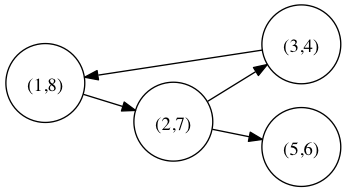
\includegraphics[width=.7\textwidth]{9-3.gv.png}
  \caption{Yet another strongly connected componets algorithm.}
\label{fig:scc}
\end{figure}

The minimal finish time is $(3,4)$, and the result of the DFS from
$(3,4)$ will make all vertices be in the same strongly connected
components which is not correct.

\pagebreak


% -----------------------------------------------------------------------------
% PROBLEM 4
% -----------------------------------------------------------------------------
\section{}

\begin{fancyquotes}
  (6 points) Exercise 22.2--6 Give an example of a directed graph
  $G=(V,E)$, a source vertex $s\in V$,and a set of edges $E_{\pi}\subseteq
  E$ such that for each vertex $v\in V$,the unique simple path in the
  graph $G'=(V,E_{\pi})$ from $s$ to $v$ is a shortest path in $G$,
  yet the set of edges $E_{\pi}$ cannot be produced by running BFS on
  $G$, no matter how the vertices are ordered in each adjacency list.
\end{fancyquotes}

\begin{figure}[hp]
  \centering
  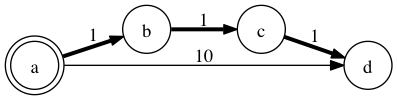
\includegraphics[width=.7\textwidth]{9-4.gv.png}
  \caption{BFS for shortest path}
  \label{fig:bsp}
\end{figure}

$G$ is showed in graph~\ref{fig:bsp}, which the bold edges are in
$E_{\pi}$.

BFS starts with $a$, after first level search, $b$ and $d$ are both
marked as searched, and $d$ will never be updated again, no matter the
order is. So $a\rightarrow d$ will always be added to the result,
which is not inside of $E_\pi$.

\pagebreak

\end{document}
